\section{Fourier equivalence and exact information limits}\label{sec:equivalence}
\subsection{Independent implementations, equivalent information}
Let $y=(\mu,\operatorname{Re}z_U,\operatorname{Im}z_U,\operatorname{Re}z_L,\operatorname{Im}z_L)$, where $z_j$ sums the completed moments \eqref{eq:event} at port $j$. The moment implementation updates only that port. Its direct readout uses a cross product; conversion to directional coordinates is not imposed merely to make a comparison.

\begin{theorem}[Invertible coordinates and conditioning]\label{thm:transform}
The relation $x=\Tp y$ is induced by
\begin{equation}\label{eq:M}
 \begin{pmatrix}u_+\\u_-\end{pmatrix}
 =\Mat\begin{pmatrix}z_U\\z_L\end{pmatrix},\qquad
 \Mat=\begin{pmatrix}e^{\ii\chi_U}&e^{\ii\chi_L}\\
                         e^{-\ii\chi_U}&e^{-\ii\chi_L}\end{pmatrix}.
\end{equation}
Its determinant is $-8\ii\sqrt3/7$ and its singular values are $4/\sqrt7$ and $2\sqrt3/\sqrt7$. The harmonic condition number is $2/\sqrt3$. The real five-coordinate transform has singular values $1$, $4/\sqrt7$ twice and $2\sqrt3/\sqrt7$ twice, and condition number $4/\sqrt7$.
\end{theorem}
\begin{proof}
Write $C=\cos\theta=\sqrt{3/7}$, $S=\sin\theta=2/\sqrt7$. Then
\[
 \Mat=\begin{pmatrix}-C+\ii S&-C-\ii S\\-C-\ii S&-C+\ii S\end{pmatrix},
 \qquad\det\Mat=-4\ii CS=-8\ii\sqrt3/7 .
\]
The orthonormal symmetric/antisymmetric vectors diagonalize this normal matrix with eigenvalues $-2C$ and $2\ii S$. Singular values are their moduli. The interleaved harmonic real block is
\[
 \begin{pmatrix}
 -C&-S&-C&S\\ S&-C&-S&-C\\
 -C&S&-C&-S\\-S&-C&S&-C
 \end{pmatrix}.
\]
Realification repeats each complex singular value twice: a singular vector and its multiplication by $\ii$ span the corresponding real plane. The mean is an independent identity coordinate. Both harmonic singular values exceed one, so the full maximum/minimum ratio is $4/\sqrt7$. Nonzero determinant supplies the inverse.
\end{proof}
This exact information equivalence precedes nonlinear projection. Independent implementations can have different instruction counts; a change of basis does not create information or prove an algorithmic advantage.

\begin{proposition}[Direct moment readout]\label{prop:momentread}
With $w=z_U\overline{z_L}$, the numerator and denominator of $\etaosc$ are
\begin{equation}\label{eq:momentread}
 \begin{aligned}
 N_{\rm dir}&=4\sin(2\theta)\operatorname{Im}w,\\
 D_{\rm dir}&=2(|z_U|^2+|z_L|^2)+4\cos(2\theta)\operatorname{Re}w .
 \end{aligned}
\end{equation}
The denominator is positive for a nonzero pair of moments.
\end{proposition}
\begin{proof}
Expand both squared moduli in \eqref{eq:M}. Diagonal terms cancel in the difference and add in the sum. The two cross phases are $e^{-2\ii\theta}$ and $e^{2\ii\theta}$; their real-part difference is $2\sin(2\theta)\operatorname{Im}w$ and their sum is $2\cos(2\theta)\operatorname{Re}w$. The factor two from each modulus expansion gives the formulas. Positivity follows from $D_{\rm dir}=\norm{\Mat z}^2$ and invertibility.
\end{proof}

\subsection{Isolated order is periodic information}
\begin{theorem}[Isolated timing domain]\label{thm:isolated}
For one positive-amplitude completed pulse at each port, from zero preparation, $\operatorname{sign}\etaosc=\operatorname{sign}\sin(2\pi(d_L-d_U))$. This equals actual onset order for $0<|d_L-d_U|<1/2$. Simultaneity and half-period lags have zero numerator. Periodic aliases prevent extension to unrestricted onset differences.
\end{theorem}
\begin{proof}
Equation~\eqref{eq:event} gives
$z_U\overline{z_L}=B_1^2A_UA_Le^{2\pi\ii(d_L-d_U)}/16$.
The factor $4\sin2\theta$ and the denominator are positive. Sine has the required sign on $(-\pi,\pi)$, vanishes at integer multiples of $\pi$ and is periodic. For instance, positive lag $3/4$ gives a negative sine, while lag one gives zero. The restriction is mathematical, not a numerical defect.
\end{proof}
If one amplitude is zero, there are not two detected events whose order the feature can infer. The timestamp comparator uses the actual onset difference and its arithmetic tolerance; it is not restricted by phase periodicity.

\subsection{Aligned streams: majority, collision and mean growth}
A lower-late quarter pair, LQ or $\ell=+1$, places $U$ at $4m$ and $L$ at $4m+1/4$. UQ, $\ell=-1$, exchanges ports. All amplitudes are one and no reset occurs between pairs. Write $N_+,N_-$ for label counts, $N=N_++N_-$ and $D_N=N_+-N_-$.

\begin{theorem}[Aligned majority formula]\label{thm:majority}
Under these alignment, amplitude and quarter-lag hypotheses,
\begin{equation}\label{eq:majority}
 u_\pm=\frac{B_1}{4}(1-\ii)(NC\pm D_NS),\qquad
 \etaosc=\frac{4\sqrt3\,N D_N}{3N^2+4D_N^2}\quad(N>0).
\end{equation}
The feature gives the majority order, with a tie at $D_N=0$, and need not give the last order.
\end{theorem}
\begin{proof}
Put $c_0=B_1C/4$, $s_0=B_1S/4$. Substitution into \eqref{eq:event} gives LQ increment $(1-\ii)(c_0+s_0,c_0-s_0)$ and UQ exchanges its components. Integer-period translations leave them unchanged. Summing the two counts proves the first identity. Since $|1-\ii|^2=2$, the difference/sum of $(NC\pm D_NS)^2$ gives $2ND_NCS/(N^2C^2+D_N^2S^2)$, which reduces to the second. Its positive denominator leaves the sign of $D_N$.
\end{proof}

\begin{corollary}[Latest-order obstruction]\label{cor:collision}
The histories $[\mathrm{LQ}@0,\mathrm{UQ}@4]$ and $[\mathrm{UQ}@0,\mathrm{LQ}@4]$ have the same exact five-coordinate lossless state and last-completion metadata but different final labels. No deterministic decoder of those data can recover both final labels.
\end{corollary}
\begin{proof}
Both have $N=2,D_N=0$, $\mu=2$ and $u_+=u_-=B_1C(1-\ii)/2$. Their last completion is $4+1/4+1=21/4$. All allowed decoder inputs coincide, so its outputs coincide, while the required final labels are opposite.
\end{proof}
This is an obstruction for the commutative exact aggregate, not a theorem against all nonlinear encoders or an associative-memory capacity bound. Floating residues between theoretically identical histories are not robust stored labels.

Each pair adds one to $\mu$, so the mean account is $N^2/2$, equal to $8192$ at $N=128$. It is not $N$ independent slots. During the retained idle queries at extra delays $0,1,10^3,10^6$ periods the coefficients remained byte-identical. The maximum phase and output discrepancies were $1.99\,10^{-10}$ and $6.45\,10^{-10}$: effects of binary64 query-clock/argument reduction, not a million executed dynamical updates.

\begin{figure}[ht]
\centering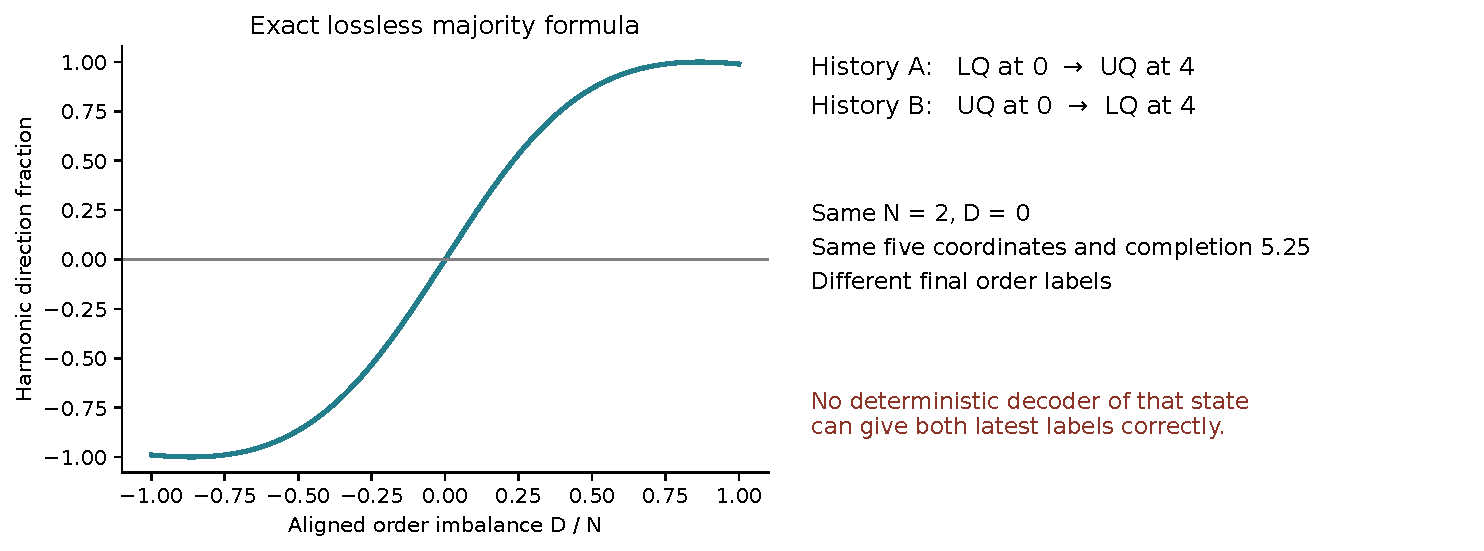
\includegraphics[width=\linewidth]{figures/fig02_aggregate.pdf}
\caption{Exact aligned aggregation. The curve illustrates the formula in $D_N/N$; finite counts occupy a discrete subset. The collision retains identical state and completion time but opposite final labels.}
\label{fig:aggregate}
\end{figure}
